\chapter{Method}\label{Method}

This section will go through an overview of the design choices that were made throughout this project on various levels in order to ultimately achieve the previously laid out research objectives (Chapter \ref{Introduction}). These design choices can be grouped into three different categories: Data Gathering, Sentiment Analysis and Statistical Analysis. Each of which will be explained in detail in the paragraphs below. The system that was built as part of this study includes pieces built specifically for this project as well as a number of existing technologies. An overview of the entire system and those technologies can be found in Figure \ref{system figure}, each of these pieces are further explained in the sections below. The system was built using the Python\footnote{\url{https://www.python.org/}} programming language and the corpus was loaded into a MySQL database.


\begin{figure}[h!]
      \centering
      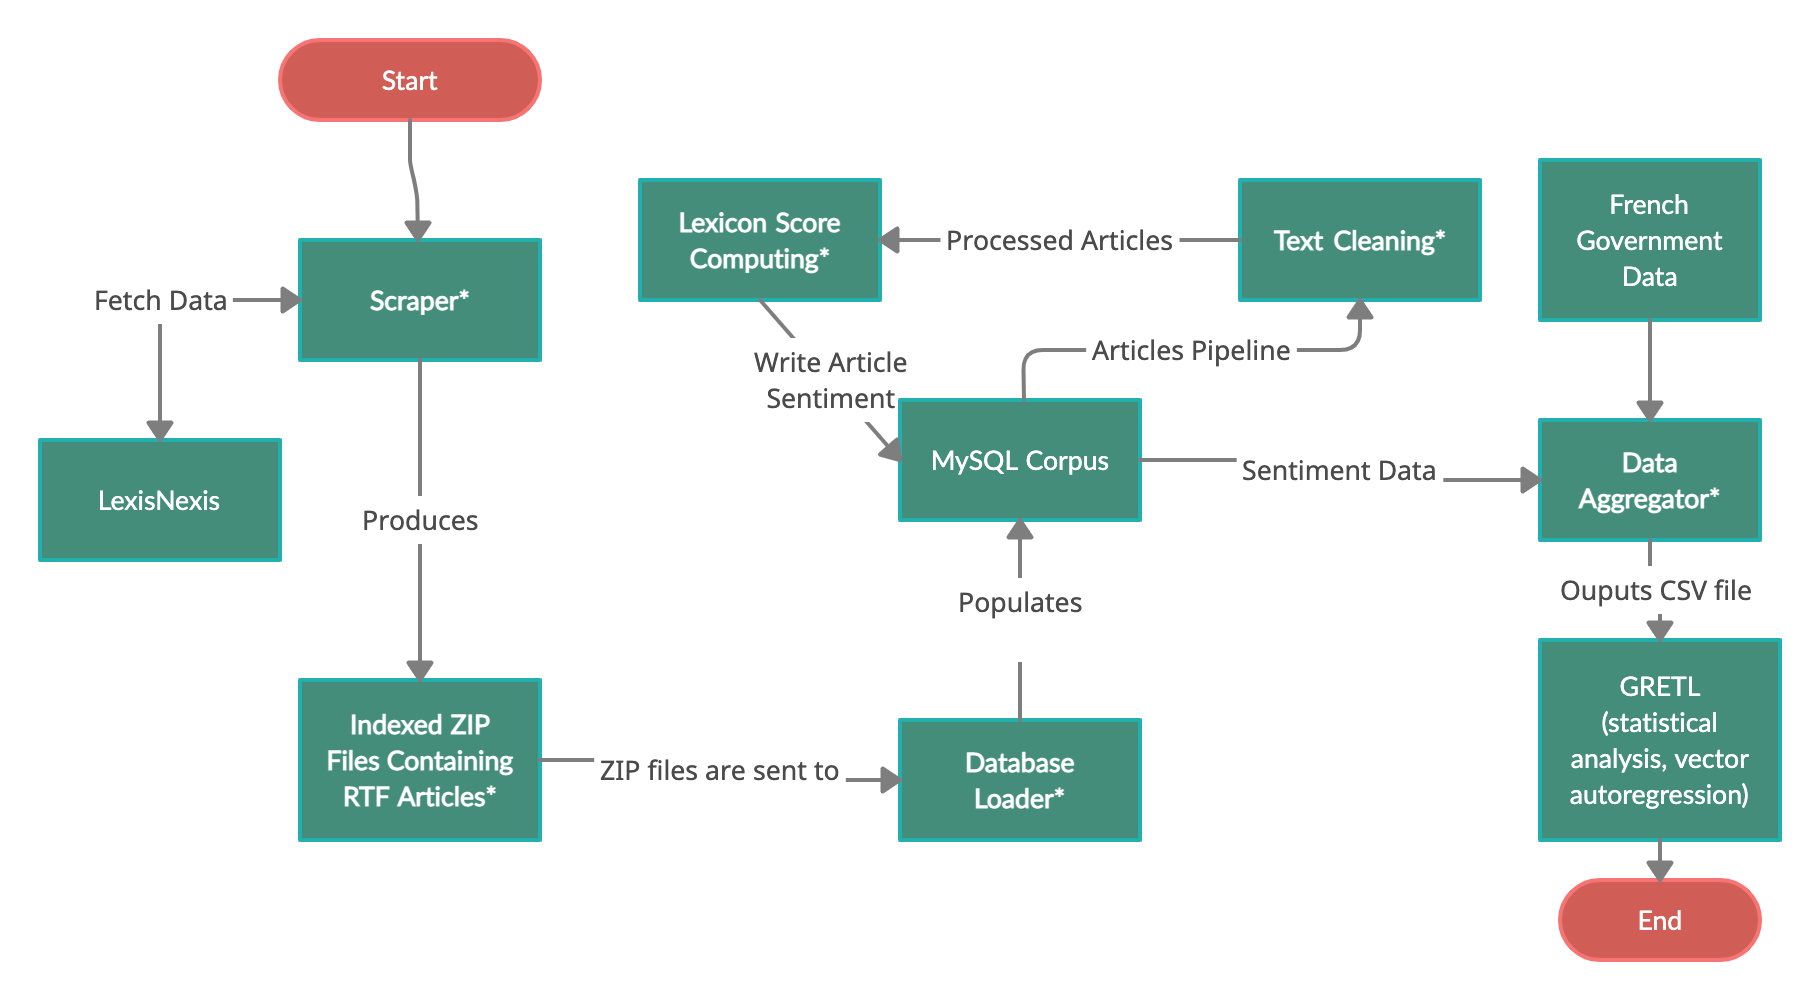
\includegraphics[scale=0.23]{method/system_1.png}
      \caption{System Overview}
      \label{system figure}
      \emph{* indicates a module that was built as part of this thesis, the remaining modules integrate the specified technologies in the system}.
\end{figure}

\section{Data Gathering}

The first part of this subsection addresses the process of identifying, gathering and organising data such as to create a quality corpus and ultimately achieve the research objective: \emph{Gather a large corpus containing high quality French news articles relevant to COVID-19}.

\subsection{Relevant Articles of Quality}

This section provides answers to the following questions about creating this data set:
\begin{enumerate}
    \item What makes an article relevant for the corpus?
    \item How to ensure the quality of the corpus?
    \item When should the start and end date for data collection be?
\end{enumerate}

\subsubsection{Relevancy}

An important part of gathering data is making sure of the data's relevancy, which validates that the corpus to be built will be ultimately useful and for the results to be relevant. In order to build a relevant corpus, articles must show relevance to COVID-19. To verify an article's relevancy, the mention of "covid", "corona", "COVID-19" or "coronavirus" in an article is sufficient to label an article as relevant.

A second variable important to building this corpus is timing. Articles are only relevant if they occured within the time window of the COVID-19 pandemic. According to the WHO\footnote{\url{https://www.who.int/news/item/29-06-2020-covidtimeline}}, the first COVID-19 event worldwide dates from the 31st of December 2019. The corpus was built using a time range from the 1st January 2020 until the 25th March 2021 which is the date when data collection was finished. It may look at first like the 31st December 2019 should have been included in the range, it turns out that the data shows the first month of events was not reported much in French news articles, in fact it represents less than $0.005\%$ of the articles in the corpus with the first article being published on the 2nd of January 2020 and the second one on the 10th.

Final details to ensure relevancy include making sure that the publication language is in French as well as the publication location to be in France.

\subsubsection{Quality Articles}

A large amount of articles are written continuously on many different platforms such as social media, news platforms or web blogs for example. This study will focus on French news articles as they play a major role in distributing information to the general public. The \emph{Alliance pour les chiffres de la presse et des médias} (ACPM)\footnote{\url{https://www.acpm.fr/Les-chiffres/Observatoire-2020-de-l-ACPM-Syntheses-2019}} is a non-profit organisation which verifies the distribution of French newspapers. The ACPM recorded an average of 9 million physical articles diffused and 60 million online visits daily in their 2020 review. To put these numbers into perspective, the \emph{Institut national de la statistique et des études économiques} (INSEE)\footnote{\url{https://www.insee.fr/fr/statistiques/1892117?sommaire=1912926}}, the national statistics bureau of France, recorded a total population of 67 million in 2020. Analysing these articles is thus particularly interesting given the large fraction of the population who are reading them. It is also worth noting that articles published by reputable sources are written by professionals, fact checked and verified on multiple levels within a news organisation before getting published. By targeting reputable French news sources, it is then expected to obtain a corpus containing high-quality, professionally written articles. It is important to make sure that any selected source is of sufficient quality as outlined above. Because of this, online blogs and sites have not been included in the corpus as they do not meet the quality threshold. These sources have been found to heavily reference themselves and rely on other news sources \cite{adamic2005political}. To further ensure quality, the sources of this corpus have all made a licensing agreement with LexisNexis News \& Business.

\subsubsection{Duplicates}

Methods were originally put in place to identify and remove duplicate articles by computing a ratio of similarity. After some considerations duplicate articles were kept in the corpus for multiple reasons.

Firstly, it is worth clarifying what is meant by duplicate articles: an article that has been published by a individual source will not be included twice in the corpus. Duplicates here are articles that may be published multiple times by different sources. For example a news organisation may be publishing multiple regional news editions which may include the same or a slightly modified version of the same content. Hence while one original writing was published multiple times, it was done so by different sources.

By keeping those duplicate articles, the corpus represents more accurately the flow of information being made available to the public by news organisations. The repetition of a story in different sources reflects its importance and not including articles from certain sources because of a duplicate article would bias any source-specific analysis.

Doing so removes the need for deduplication which is a challenge of its own. News articles are rather large in nature and computing string similarity ratios for each pair of articles can be very expensive to compute.

\subsection{Large Data Collection}\label{Data Collection}

With regards to how big the corpus should be, there are three questions to answer:
\begin{enumerate}
    \item How many articles should be gathered?
    \item How many articles should be retrieved per source?
    \item How to gather articles and structure the corpus?
\end{enumerate}

\subsubsection{Corpus Size Assessment}

It is important to build a corpus of a substantial size such as to avoid any potential biases which can occur with small sample sizes. It is also important to include both national and regional publications. While some types of regional publications consist mostly of national news, most regional publications are found to differ significantly in content when compared to national publications \citep{ballarini2008presse}. France is home to hundreds of different news sources, when considering all the different type of news publications such as daily, weekly, biweekly, monthly and more. Over 200 of which have business agreements with LexisNexis News \& Business. This makes for a sufficient selection of sources for this corpus.

With regards to the quantity of articles to gather per source, the goal is to retrieve as many articles per source matching the relevancy criteria. LexisNexis makes it possible to retrieve all of the articles matching the relevancy criteria for the selected sources which removes the need of selecting a random sample. This will enable analysis on which sources publish the most COVID-19 related articles as well as the variations in the amount of articles published over key events or periods. It is worth noting that this may introduce a bias in other analyses as some sources publish much more than others, it remains however necessary for the corpus built to be large enough.

To summarize, the corpus will be built by gathering as many articles as possible that match the relevancy criteria and come from a set of selected sources. As many sources as possible will be selected, given that they match the quality standard discussed above and have a licensing agreement with LexisNexis \& Business.

\subsubsection{Collecting Data}\label{Collecting Data}

A small corpus was originally built by manually downloading articles matching the previously laid out relevancy filters from LexisNexis, it quickly became apparent that such an approach would not be sufficient to build a corpus large enough for this study.

A scraper was built instead to automate the process of downloading those articles. A total of 369,569 articles listed on LexisNexis match the selected filters. As a service, LexisNexis enables downloading articles in batches of up to 500. It also enables options into the formatting of documents such link embedding, text formatting and more. As part of this system, the documents will be downloaded in rich text format (RTF), references will not be embedded as links such as to simplify the document parsing process, and articles will be saved as individual files which will be compressed as a ZIP file grouping 500 articles each. Note that all of these are options to be set by the scrapper on the options dialog before triggering a download.

The technologies used to build the scraper include the Google Chrome browser, its associated "ChromeDriver"\footnote{\url{https://chromedriver.chromium.org/}} which enables triggering browser actions programmatically, the Python programming language and finally Selenium. Selenium\footnote{\url{https://www.selenium.dev/}} is an open-source framework which makes performing automated browser actions easier. Figure \ref{fig:scraper pseudo code} shows a simplified set of actions performed by this scraper in pseudo code format:

\begin{figure}[H]
\centering
\begin{BVerbatim}
load_url()
login()
handle_pop_ups()
while !finished_downloading() {
    open_download_dialog()
    enter_download_parameters()
    trigger_download()
    wait_for_download_triggered()
    wait_for_download_finished()
    rename_and_index_downloaded_file()
}
\end{BVerbatim}
\caption{Simplified Scraper Pseudocode}
\label{fig:scraper pseudo code}
\end{figure}

There were a few issues specific to LexisNexis that needed solving before having a working, independent scraper. The first one was dealing with pop-ups. Opening LexisNexis from a scrapper with no cookies will open 0 to 3 different pop-ups promoting various events. To avoid scrapers these pop-ups include an automatically generated id in their HTML tag which made it harder to close automatically, their load time varied heavily as well. To solve this issue, a time period of 60 seconds on page load was put in place. During that time the system attempts to identify any pop-up HTML component and identify any buttons within the component. Such pop-ups only include close buttons which made the closing task easier.

Another issue that was later discovered is that downloading articles from LexisNexis requires a range of articles to download, for instance a range of 1-500 would download the first 500 articles matched. The issue came when using an offset greater than 30,000 (for example a range of 30,001 - 30,500) which broke LexisNexis' download system and no download would be triggered. To solve this issue, batches of a maximum of 30,000 articles were created manually. The process for doing so was:
\begin{enumerate}
    \item Manually log into LexisNexis and set the search filters.
    \item Select a time range such that the total returned articles is below 30,000.
    \item Copy a permanent link URL such that the scraper can load load the URL with the filters and time range already set. Also copy the total number of articles.
    \item Repeat the process such that the whole time range is covered. It is very important to make sure not to include date overlaps as doing so would introduce duplicate articles.
\end{enumerate}

From this process a set of URLs as well as their associated article counts are obtained. The scrapper can now iterate through these batches and download all the targeted articles.

Another issue the scrapper ran into was rate limiting. The university limits how many downloads one account can make over a certain period of time. When that limit is reached, the account is blocked from accessing LexisNexis for two hours. The only solution for this was to have the scraper identify the rate-limiting web page and to let the script sleep for two hours when the event occurs.

Finally, it was crucial for the scrapper to be able to handle unexpected errors gracefully. Given that it was executed for a time period of 7 days in total, unexpected network errors and many others could occur. Hence before starting to download articles, a check is performed in the directories containing previously downloaded files such as to identify which batches are complete and which ones are not. That way the scraper can resume work where it left off in case of any error.

Running this system for a week was sufficient for the system to download all of the 369,569 articles that matched the previously selected set of filters.

\subsubsection{Organising Data}

This section will include details on how the scraper system organises downloaded files as well as how the downloaded articles were aggregated to enable easy and fast operations.

Once a download finished successfully, the scrapper moves that file from the download directory to the output directory matching the current batch of articles being downloaded. The output directories include all of the indexed files that were previously downloaded. When moved to an output directory, the files are renamed to include information about the batch they come from as well as the offset used to obtain this file. This indexing enables the scraper to keep track of which files have and haven't been downloaded, hence making sure that no individual article is downloaded twice.

The next task is to extract relevant information from the 740 ZIP files, containing 369,569 individual articles that were downloaded by the scraper. A MySQL database was used to organise the corpus as it enables easy and fast operations that wouldn't be possible otherwise.

The process of loading the data into a structured, relational database also required important design choices. Similar to the scrapper, care must be placed in loading each article no more than once, and, given the amount of data to be handled, the system must be able to resume work on error. The procedure for loading data is detailed in Figure \ref{database loader}. The approach writes important data to text files to keep track of which ZIP file is currently being processed and a separate file to keep track of the list of ZIP files which have been already loaded. By doing so the system knows at all times what work has been done and what is remaining, hence enabling the system to crash and resume work where it left off. The final detail is that after a specific RTF file containing a single article was parsed and loaded into the database, that file is deleted to make sure not to load it twice.

\begin{figure}[H]
      \centering
      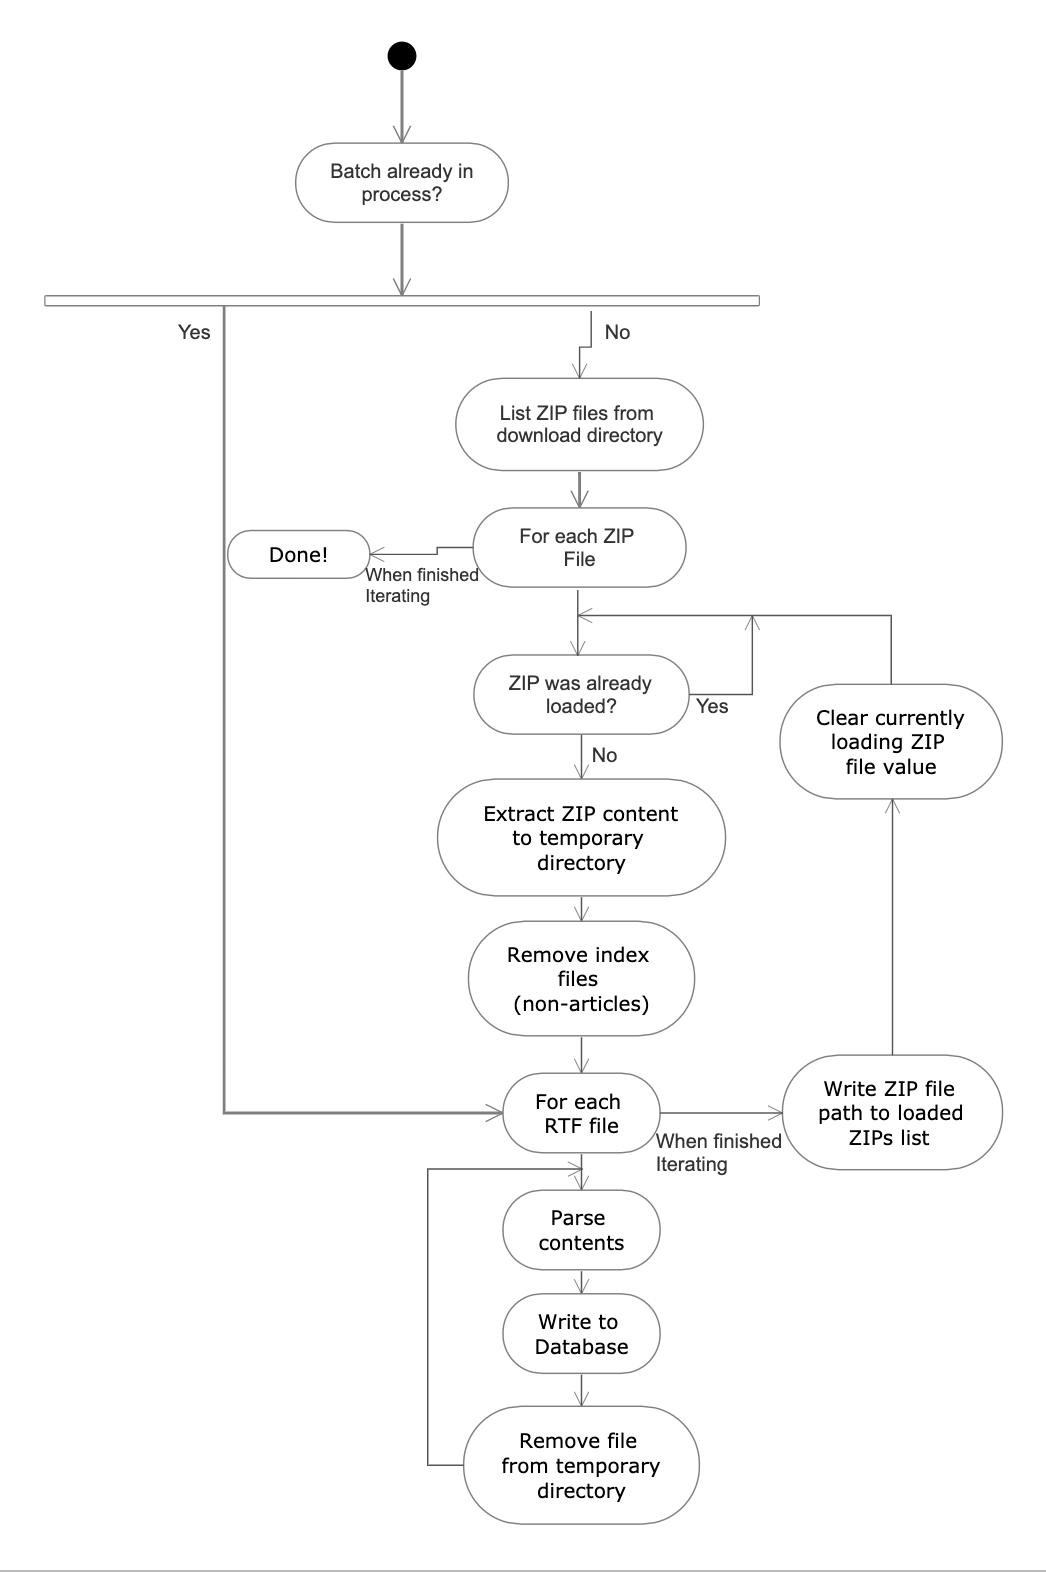
\includegraphics[scale=0.7]{method/db_loader.png}
      \caption{Loading Articles Into MySQL}
      \label{database loader}
\end{figure}

Finally, the articles come in rich text format (RTF). The content parsing algorithm parses and splits the RTF text into various sections:
\begin{enumerate}
    \item Article title
    \item Source
    \item Date
    \item Copyright
    \item Body
    \item Author
\end{enumerate}

More information is extracted however the above fields represent the most important data points to be used throughout this study. To conclude this section, it is worth noting that a number of articles did not include a date, or was formatted differently than the parser expected. In these instances, the article was not loaded into the database as the timing of an article was deemed important to this study.

\section{Sentiment Analysis}

The following subsection will cover the sentiment analysis part of this study. Including both the dictionaries used as well as the sentiment analysis pipelines. It addresses the following two research objectives: \emph{Create specialised dictionaries targeted to measure pandemic-related sentiments} as well as \emph{Perform sentiment analysis on the corpus to retrieve measures for various sentiments and term frequencies}.
 
\subsection{Specialised Dictionaries}\label{Custom Dicts}

The vocabulary typically used in news articles is very general, by using a simple vocabulary, a news article ensures that its readers will understand the content provided. More generally, journals use a vocabulary that is familiar to its readers, with the exception of topic-specific sources covering subjects such as finance or sports for example, the vocabulary for the sources analysed in this study is quite general and easy to understand. As a newly emerging disease such as COVID-19 is discovered, news papers are found to adopt new specialised terminology. General lexica such as FEEL (Chapter \ref{chap: feel}) may contain some specialised terms and associate it with a negative sentiment. This is not accurate as in the context of a pandemic, the mention of "virus" for example, should not be seen as negative. To do so, the terms of the specialised dictionaries are removed from the lexica used.

In order to extract sentiment proxies specific to the COVID-19 pandemic, three specialist dictionaries were created. These dictionaries target the mentions of virus, vaccination and death. The process for creating these three dictionaries involved the corpus analysis tool AntConc\footnote{\url{https://www.laurenceanthony.net/software/antconc/}}. AntConc enables the analysis of word patterns within a corpus, a manual selection of terms from the analysis performed in AntConc yielded the three dictionaries.

\subsubsection{Virus}

The Virus dictionary is the largest lexicon out of the three as it is also the most vast. The aim of this lexicon is to enable the measurement of virus-related words. It consists of words, expressions and objects that have been made popular or used in the context of the COVID-19 pandemic. The total lexicon includes seventy five words, Table \ref{tab:virus lexicon} shows twenty five entries. Care was put in reducing overlap between the three dictionaries, since this one was the largest, death and vaccination related terms have not been included in this lexicon.


\begin{table}[H]
\centering
\begin{tabular}{@{}llll@{}}
\toprule
\multicolumn{4}{c}{\textbf{Virus Lexicon}} \\ \midrule
administration test & covid-19 & geste barrière & pandémie \\
antibiotique & distanciation social & hospitalisation & pandémique \\
aplatir courbe & déconfinement & immunisation & pathogène \\
asymptomatique & déconfiner & immuniser & patient zéro \\
auto-immun & déconfiné & immunité & pneumonie \\
auto-isolement & déficit immunitaire & immunodéprimé & quarantaine \\
bactérie & dépistage & infecter & restriction \\
cas actif & dépister & infection & réanimation \\
cas confirmer & désinfectant & insuffisance respiratoire & symptôme \\
cas confirmé & désinfecter & isolement & taux de mortalité \\
cas contact & epidémie & isoler & test antigénique \\
charge viral & epidémiologie & laver main & transmission \\
clinique de dépistage & faux négatif & lits soins intensifs & viral \\
confinement & faux positif & masque & virologie \\
confiné & fermeture frontière & mesure sanitaires & virus \\
contamination & fièvre & mutation & vulnérable \\
contaminer & foyer infection & muter & écraser courbe \\
coronavirus & germe & nasal & épidémie \\
couvre-feu & germes & \textit{oms} & \\
\bottomrule
\end{tabular}
\caption{Virus Lexicon}
\label{tab:virus lexicon}
\end{table}

\subsubsection{Vaccine}

Similarly, this lexicon aims to quantify the presence of vaccination-related words in articles, consisting of words specific to the vaccination field as well as the names of COVID-19 vaccines or companies producing them. It contains  twenty eight words which are displayed in Table \ref{tab:vaccine lexicon}.

\begin{table}[H]
\centering
\begin{tabular}{@{}ll@{}}
\toprule
\multicolumn{2}{c}{\textbf{Vaccine Lexicon}} \\ \midrule
adjuvant & injection \\
administrer & \textit{janssen} \\
anticorps & \textit{johnson\&johnson} \\
antigène & \textit{moderna} \\
antiviral & pathogène \\
arn & \textit{pfizer} \\
\textit{astrazeneca} & \textit{sanofi} \\
\textit{biontech} & \textit{spoutnik v} \\
\textit{curevac} & vaccin \\
dose & vaccinal \\
immunisation & vaccination \\
immuniser & vacciner \\
immunité & \textit{vaxzevria} \\
immunoglobine & virologue \\
\bottomrule
\end{tabular}
\caption{Vaccine Lexicon}
\label{tab:vaccine lexicon}
\end{table}

\subsubsection{Death}

This final lexicon targets the mention of death within an article, it consists of sixty five words in total which are shown in Table \ref{tab:death lexicon}.

\begin{table}[H]
\centering
\begin{tabular}{@{}lll@{}}
\toprule
\multicolumn{3}{c}{\textbf{Death Lexicon}}    \\ \midrule
agonie        & ensevelissement & mort           \\
avoir quitter & enterrement     & mortel         \\
cadavre       & enterrer        & mourant        \\
caveau        & extinction      & mourir         \\
cendres       & exécution       & obsèques       \\
cercueil      & fatal           & pierre tombale \\
cimetière     & fossoyeur       & périr          \\
commémoration & funeste         & ressusciter    \\
condoléances  & funèbre         & résurrection   \\
crypte        & funérailles     & succomber      \\
crématoire    & funéraire       & sépulture      \\
crématorium   & génocide        & s’éteindre     \\
cénotaphe     & homicide        & tombe          \\
deuil         & hôpital         & tombeau        \\
disparaître   & incinération    & trépas         \\
disparition   & incinérer       & trépasser      \\
décimer       & inerte          & tuer           \\
décès         & inhumation      & victime        \\
décéder       & lugubre         & âme            \\
défunt        & maladie         & épitaphe       \\
dépouille     & martyre         & éteindre       \\
ensevelir     & meurtre         &                \\ \bottomrule
\end{tabular}
\caption{Death Lexicon}
\label{tab:death lexicon}
\end{table}
\subsection{Sentiment Analysis Pipeline}

Originally the text analysis software Rocksteady \citep{ahmad2014rocksteady} was used. Rocksteady is a lexicon based affect analysis system which was developed in Trinity College Dublin, Ireland. Once the scraper system (Chapter \ref{Collecting Data}) was put in place it became apparent that a more flexible system was required. Rocksteady requires the aggregation of articles into text files which comes with limitations, handling 369,569 articles in the form of text files is very expensive, whether it is to aggregate the corpus into a single or many files such that Rocksteady can read the corpus, reading all of that data on each load, computing all of the sentiments for the whole corpus at once which could run into memory issues as attempting to compute sentiment for a large amount of articles requires a flexible system such that sentiment can be computed through a data pipeline. In light of this, the articles were parsed, organised and loaded into a MySQL database as described in Chapter \ref{Collecting Data}. Using a MySQL system also enables extremely fast article retrieval as well as very useful data aggregation methods such as date grouping, source grouping and more within seconds. The following sections explain in detail how the system was implemented.
 
\subsubsection{Lexicon Handling}

The first part of performing lexicon based sentiment analysis on an article is to first load and process the various lexica used. As part of this project three specialist dictionaries (Chapter \ref{Custom Dicts}) were used. FEEL, Diko as well as Polarimots (Chapter \ref{French Lexicons}) are three more general lexica which were used to measure polarity as well as other emotions where possible. As previously mentioned, overlap between general and specialised lexicons was removed from the general lexicons.

With regards to the custom dictionaries, the process for loading each lexicon was to load the text file containing the lexicon. These lexica are built in the form of one word per line. Splitting the resulting string using the new line character yields an array of all of the words within that lexicon. No weight was associated for each of the words so the count of occurrences within an article was used as the final score for each lexicon.

FEEL, Diko and Polarimots required more processing. Each of these lexicons had specific requirements when it came to putting it into practise as some included specific emotions and details. The following sections will explain how weights were applied for each of these dictionaries.

The FEEL lexicon includes for each word a polarity (negative or positive) as well as a value of 1 or 0 for the following emotions: joy, fear, sadness, anger, surprise and disgust. For this lexicon a similar approach to the custom dictionaries was used: a count of occurrences for each of the emotions as well as the polarity occurrences.

The Diko Lexicon includes for each word a number of vote for its polarity (negative, positive, neutral). These votes were used to compute a score for each word, the following points were taken into account:
\begin{enumerate}
    \item Amount of total votes relative to the entire lexicon
    \item Positive / negative vote frequency
    \item Neutral votes: a large number of neutral votes pushes the score towards 0
\end{enumerate}
To do so, the following value is computed:
\begin{equation}
    \frac{\#pos - \#neg}{\#pos + \#neg + \#neut}
\end{equation}
This scoring system works as it reflects the positive or negative frequency of votes relative to the total amount of votes. It is also important that more positive votes yields a positive score and on the contrary a negative score which is the case with this function. However it does not reflect an accurate score with regards to how many votes were observed relative to the entire lexicon. For example, a word with 10\% of positive votes, 80\% negative and 10\% neutral will have the same score if it has a total vote count of 10 or 10000. This needs to be taken into account as a reliability measurement.
To do so, we start by computing the Z-Score for the total vote counts, which measures how far apart from the mean a data point is:
\begin{equation}
    \frac{(\#pos + \#neg + \#neut) - \mu}{\sigma}
\end{equation}
Where $\mu$ is the mean for total votes on the lexicon and $\sigma$ is its standard deviation. This measure provides a reliability metric as previously discussed, however it comes with the issue of returning a negative value when the total word count is below the mean which is an issue for the final score. By not subtracting the mean in the Z-Score and multiplying both measures together, we obtain the weight function for this dictionary:
\begin{equation}
\label{diko score}
    score = \frac{\#pos - \#neg}{\#pos + \#neg + \#neut} * \frac{(\#pos + \#neg + \#neut)}{\sigma}
\end{equation}
Where $\#neg$, $\#neut$ $\#pos$ is the number of negative, neutral and positive votes respectively for a word entry, $\sigma$ is the standard deviation for total votes in the lexicon.

One final detail is that the Diko dictionary is very large, containing over 1.2 million word entries. Using the entire dictionary is not of much use and unrealistic on a large corpus. To solve this, words with a total vote count below 500 were skipped as well as words with scores in the range of $-1 < score < 1$. This returns a total of 24,643 words to use from this lexicon.

Last but not least, the Polarimots dictionary includes for each word a polarity which can be one of neutral, positive and negative. Also associated with each word is a reliability metric of either 100\% 66\% or 33\%. This reliability metric was divided by 100 such as to obtain 0.33, 0.66 and 1 which makes for the weights used with this dictionary.

\subsubsection{Data Pipeline}

Given the large quantity of articles in this corpus. A data pipeline feeding articles to the sentiment analysis system is required such as not to load all of the articles at once. Articles are loaded in batches of 2000, once a batch is finished processing the resulting sentiment computed is saved into the database. The algorithm then ends once all of the articles sentiments have been saved to the database.

It was very important to save sentiment outputs to the database for two main reasons:
\begin{enumerate}
    \item Computing sentiment on the corpus for each lexicon took between 10 to 16 hours depending on the size of the lexicon used. Being able to proceed by batch and resume on error is valuable.
    \item Storing sentiment values in an articles metadata enables further analysis grouping or filtering articles within seconds by using the already computed sentiment values.
\end{enumerate}

\subsubsection{Text Cleaning}

Articles are put through a series of steps that modify them in some way in order to compute sentiments in the best of conditions. First, the articles are converted to lowercase, this step is not always necessary but the lexica used all use lowercase words. The second step is to remove stop words and punctuation. The list of stop words used come from SpaCy's French language pipeline (Chapter \ref{lemmatization}). Finally, the remaining words are lemmatized also using SpaCy.

\subsubsection{Computing Sentiment}

This final step receives a processed and cleaned text and outputs a set of sentiment scores. The first step to do so is to count the occurrences of the lexicon words within the article. While originally a set of nested for loops were put in place to do so. After some brief manual experiments, using regular expressions was found to be much faster. Hence from a provided lexicon, a single regular expression is compiled. The regular expression matches the pattern seen in Figure \ref{fig:regex}.

\begin{figure}[H]
\centering
\begin{BVerbatim}
(\bhello\b|\bworld\b)
\end{BVerbatim}
\caption{Regular Expression with Two Terms}
\label{fig:regex}
Lexicons were mapped to a regular expression of this format in order to find occurrences within news articles.
\end{figure}

The parentheses mark the group of the regular expression, the above expression would match the words "hello" and "world". Notice that they are wrapped in $\backslash$ followed by "b", this operator in regular expressions makes sure to only match entire words, hence verifying that a white space character is present before and after the word within the article. The final detail is that all of the lexicon's words are separated by a "|" operator which is the equivalent of the "OR" operation in a regular expression.

Using a lexicon's compiled regular expression as described above, we obtain a set of paired values, including a subset of the lexica words and its associated number of occurrences within the article.
All that is left is to iterate through those matches, for each word retrieve the associated weight, make sure to multiply it by the number of occurrences and keep a running total of all of the sentiments included within the lexicon used.

Some sentiment systems will act as a classifiers, whether it is machine learning or lexicon based, by returning "positive" or "negative" for a specific article. This system does not and keeps both the positive and negative scores obtained from an article, it provides more details useful to the statistical analysis.

\subsection{Output Aggregating}\label{chap: output aggregating}

The final step of the sentiment analysis system is to format the output such that it can be used for statistical analysis. To do so, information about the corpus as well as its computed sentiment scores are grouped daily and retrieved from the database. Official data from the French government\footnote{\url{https://www.data.gouv.fr/en/datasets/donnees-relatives-a-lepidemie-de-covid-19-en-france-vue-densemble/}} is appended to the sentiment data. Metrics used from the French government include: the number of confirmed COVID-19 cases, number of deaths and the number of first vaccine injections, corresponding to the data points "casConfirmes", "deces" and "nouvellesPremieresInjections" respectively in the summary data set. This outputs a set of daily data points which includes various sentiments and official COVID-19 French metrics.

\section{Statistical Analysis}\label{chap: stat analysis}

The final subsection will cover details of the last remaining research objective: \emph{Conduct statistical analysis on the results in order to identify and quantify potential relationships}.

\subsection{Vector AutoRegression}

The tool used for statistical analysis in this project is the GNU Regression, Econometrics and Time-series Library (GRETL). It is a powerful open-source tool for statistical analysis which was picked for this project for its performance and accuracy. The process for building each model involved a few steps. They will be detailed in the following sections.

\subsubsection{Unit Root Testing}

Before any regression can be performed, it is is important to check all of the variables are stationary. This verifies that the variables statistical properties such as the mean, variance or autocorrelation are standard over time. This is done with the Augmented Dickey–Fuller (ADF) test. In the case that this test fails, the next step is to test for cointegration using Engle-Granger cointegration test. If this test succeeds, then a vector error correction model (VECM) shall be used instead of vector autoregression (VAR). If however the test fails then the variables failing are first-order differenciated.

\subsubsection{Lag Selection}

The following step is to perform lag selection, and in fact, a lag order is required to perform the above unit root testing. It is critical to select an appropriate lag length as it will heavily affect the obtained results. An incorrect lag value can result in over-fitting which is undesirable and causes an increase in the mean squared error. On the other hand, under-fitting is also undesirable and may result in autocorrelation-errors.

There are three popular approaches to optimal lag selection. Akaike Information Criterion (AIC), the Bayesian Information Criterion (BIC) and the Hannan–Quinn information criterion (HQC). All three criteria are further explained in Chapter \ref{chap:lag selection lr}. Due to the specific use cases of the three methods, lag selection will be approached on a model by model basis.

\subsubsection{Model Building}

The final step is to build VAR models. Models will be built incrementally by adding a single variable at a time.  On each iteration, a variable is added to the models and statistically significant coefficients are retrieved. The $R^2$ and adjusted $R^2$ values are computed which assesses the models performance, an increase in these values imply a higher model accuracy and on the opposite a smaller value show a decrease in the models accuracy. An F statistic and its P-value are also computed, in this situation, GRETL computes the Granger causality test as its F statistic. This test is also performed on the other direction for the newly added variable. This enables to discover whether one variable forecasts the other in both directions through the Granger causality test proxy. When no causality is found in the direction of dependent variables then that variable is dropped from the model. Finally, a Durbin-Watson test is also performed such as to detect autocorrelation. All of these statistics were further detailed in Chapter \ref{chap:var lit rv}.

\subsection{Selected Models}

Three models were built from the available variables both coming from the sentiment proxies of the built corpus as well as the French Government into a set of daily values (Chapter \ref{chap: output aggregating}). These three models were computed as they were found to be interesting, however this does not show the limits of what could be retrieved from the results of this sentiment analysis system.

\subsubsection{Death Sentiment}

This model aims to identify if there are causal relationships between the mention of death and COVID-19 metrics as well as other variables obtained from the French news media.

The first iteration of VAR for this model starts by regressing the Death Sentiment on itself. The model for this first iteration is as follows:
\begin{equation}
    DeathDict_{t} = \alpha + \beta_{1}DeathDict_{t-1} + \beta_{2}DeathDict_{t-2} + ... + \beta_{n}DeathDict_{t-n} + \epsilon_{t}
\end{equation}
\begin{equation}
    DeathDict_{t} = \alpha + \beta L_{n} DeathDict_{t} + \epsilon_{t}
\end{equation}
Where $\alpha$ is a constant, n represents the number of lags, $\beta$ the coefficient and finally $\epsilon$ is white noise. Note that both formulas are equivalent and we will be using the second, more concise formula for the remaining models.

The following step will add the daily COVID-19 death count variable (named "Deaths") to the model, it is expected that mentions of death in news paper to be correlated with the daily death count. This model is represented by the following formula:
\begin{equation}
    DeathDict_{t} = \alpha + \beta L_{n} DeathDict_{t} + \gamma L_{n} Deaths_{t} + \epsilon_{t}
\end{equation}

The next variable introduced to the model will be the virus sentiment of articles ("VirusDict"), testing the idea that a higher mention rate of the death lexicon also results in a higher rate for the virus lexicon.
\begin{equation}
    DeathDict_{t} = \alpha + \beta L_{n} DeathDict_{t} + \gamma L_{n} Deaths_{t} + \delta L_{n} VirusDict_{t} + \epsilon_{t}
\end{equation}

Then the number of daily cases ("Cases") is added into the model in order to check whether death sentiment is related to the amount of growing cases.
\begin{equation}
    DeathDict_{t} = \alpha + \beta L_{n} DeathDict_{t} + \gamma L_{n} Deaths_{t} + \delta L_{n} VirusDict_{t} + \lambda L_{n} Cases_{t} + \epsilon_{t}
\end{equation}

The negative sentiment variable ("Neg") is added to the model as it could be expected that negativity and death sentiments are correlated within the French news media.
\begin{equation}
    DeathDict_{t} = \alpha + \beta L_{n} DeathDict_{t} + \gamma L_{n} Deaths_{t} + \delta L_{n} VirusDict_{t} + \lambda L_{n} Cases_{t} + \tau L_{n} Neg{t} + \epsilon_{t}
\end{equation}

Finally, the fear sentiment variable ("Fear") is added to the model.
\begin{multline}
    DeathDict_{t} = \alpha + \beta L_{n} DeathDict_{t} + \gamma L_{n} Deaths_{t} + \delta L_{n} VirusDict_{t} \\ + \lambda L_{n} Cases_{t} + \tau L_{n} Neg{t} + \phi L_{n} Fear_{t} + \epsilon_{t}
\end{multline}
\subsubsection{Positive Sentiment}

The next model selects positive sentiment such as to identify the variables which increase the rate of positive words found in news articles. The first model used performs VAR on itself, the positive sentiment variable ("Pos").
\begin{equation}
    Pos_{t} = \alpha + \beta L_{n} Pos_{t} + \epsilon_{t}
\end{equation}

Then the variable for vaccination sentiment ("VaccineDict") is added to the model:
\begin{equation}
    Pos_{t} = \alpha + \beta L_{n} Pos_{t} + \gamma L_{n} VaccineDict_{t} + \epsilon_{t}
\end{equation}

Next, the computed value for joy ("Joy") is added to the model as positiveness and joy are expected to be positively correlated together.
\begin{equation}
    Pos_{t} = \alpha + \beta L_{n} Pos_{t} + \gamma L_{n} VaccineDict_{t} + \delta L_{n} Joy_{t} + \epsilon_{t}
\end{equation}

Finally, the rate of vaccination is added to the model ("VaccineDoses"). It is important to note that using the vaccination rate may see some varying results as vaccination in France only started on the 27-12-2020, thus leaving roughly 80\% of the date range used in this study with the vaccination rate of 0.
\begin{equation}
    Pos_{t} = \alpha + \beta L_{n} Pos_{t} + \gamma L_{n} VaccineDict_{t} + \delta L_{n} Joy_{t} + \lambda L_{n} VaccineDoses_{t} + \epsilon_{t}
\end{equation}

\subsubsection{Virus Sentiment}

The final model presented in this study focuses on the mention of virus-related terms in the French news media ("VirusDict"). To do so the first VAR model built starts on itself.
\begin{equation}
    VirusDict_{t} = \alpha + \beta L_{n} VirusDict_{t} + \epsilon_{t}
\end{equation}

The next variable introduced to the model is the number of recorded daily COVID-19 cases in France ("Cases") as a higher mention of virus terms can be expected when there are large variations in the daily cases.
\begin{equation}
    VirusDict_{t} = \alpha + \beta L_{n} VirusDict_{t} + \gamma L_{n} Cases_{t} + \epsilon_{t}
\end{equation}

Then the negative sentiment variable ("Neg") is added to the model such as to test whether more mentions of negative words is correlated to a higher frequency of the virus lexicon within articles. 
\begin{equation}
    VirusDict_{t} = \alpha + \beta L_{n} VirusDict_{t} + \gamma L_{n} Cases_{t} + \delta L_{n} Neg_{t} + \epsilon_{t}
\end{equation}

The final variable introduced to this model is the number of daily recorded deaths in order to test if a higher death rate causes the news media to mention more virus terms.
\begin{equation}
    VirusDict_{t} = \alpha + \beta L_{n} VirusDict_{t} + \gamma L_{n} Cases_{t} + \delta L_{n} Neg_{t} + \lambda L_{n} Deaths_{t} + \epsilon_{t}
\end{equation}